\documentclass[tikz,border=2mm]{standalone}
\usetikzlibrary{calc}

\begin{document}
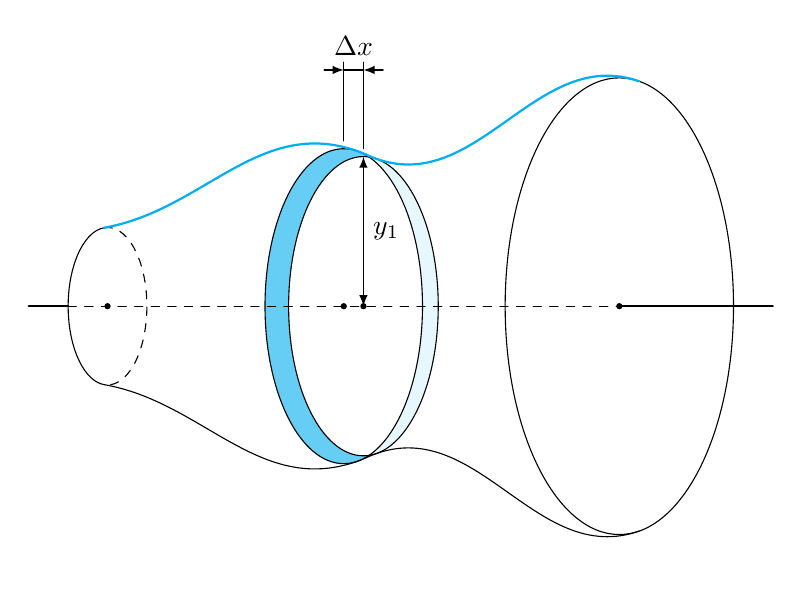
\begin{tikzpicture}[line cap=round,line join=round,xscale=0.5]
% DIMENSIONS AND COORDINATES
% first circle from the left
\def\xa{0}   % position
\def\ra{1}   % radius
\def\aa{95}  % angle
\coordinate (A0) at (\xa,0);             % center
\coordinate (A1) at ($(A0)+( \aa:\ra)$); % tangent point above
\coordinate (A2) at ($(A0)+(-\aa:\ra)$); % tangent point below
% second circle
\def\xb{6}   % position
\def\rb{2}   % radius
\def\ab{80}  % angle
\coordinate (B0) at (\xb,0);             % center
\coordinate (B1) at ($(B0)+( \ab:\rb)$); % tangent point above
\coordinate (B2) at ($(B0)+(-\ab:\rb)$); % tangent point below
% third circle
\def\xc{6.5} % position
\def\rc{1.9} % radius
\def\ac{80}  % angle
\coordinate (C0) at (\xc,0);             % center
\coordinate (C1) at ($(C0)+( \ac:\rc)$); % tangent point above
\coordinate (C2) at ($(C0)+(-\ac:\rc)$); % tangent point below
% fourth circle
\def\xd{13}  % position
\def\rd{2.9} % radius
\def\ad{80}  % angle
\coordinate (D0) at (\xd,0);             % center
\coordinate (D1) at ($(D0)+( \ad:\rd)$); % tangent point above
\coordinate (D2) at ($(D0)+(-\ad:\rd)$); % tangent point below
% DRAWING
% section
\fill[cyan!10] (B1) to[out=\ab-90,in=\ac+90]  (C1) arc (\ac:-\ac:\rc)
                    to[out=270-\ac,in=90-\ab] (B2) arc (-\ab:\ab:\rb);
\fill[cyan!60] (C1) to[out=\ab-90,in=\ac+90]  (B1) arc (\ab:360-\ab:\rb)
                    to[out=270-\ab,in=90-\ac] (C2) arc (360-\ac:\ac:\rc);
% first circle
\draw         (A1) arc (\aa:360-\aa:\ra);
\draw[dashed] (A1) arc (\aa:-\aa:\ra);
% rest of the circles
\foreach\i/\j in {B/\rb,C/\rc,D/\rd}
  \draw (\i0) circle (\j);
% surface
\draw[thick,cyan] (A1) to[out=\aa-90,in=\ab+90] (B1) to[out=\ab-90,in=\ac+90]
                  (C1) to[out=\ac-90,in=\ad+90] (D1);
\draw[yscale=-1]  (A2) to[out=\aa-90,in=\ab+90] (B2) to[out=\ab-90,in=\ac+90]
                  (C2) to[out=\ac-90,in=\ad+90] (D2);
% axis
\draw[thick]  (-\ra,0) --++ (-1,0);
\draw[dashed] (-\ra,0) --   (D0);
\draw[thick]  (D0)  --   (\xd+\rd+1,0);
\foreach\i in {A,B,C,D}
  \fill (\i0) ellipse (0.8mm and 0.4mm);
% labels
\draw[latex-latex]            (C0) --++ (0,\rc)     node[midway,right] {$y_1$};
\draw         (B0) ++  (0,\rb+0.1) --++ (0,1);
\draw         (C0) ++  (0,\rc+0.1) --++ (0,1+\rb-\rc);
\draw[-latex] (B0) ++ (-0.5,\rb+1) --++ (0.5,0);
\draw[-latex] (C0) ++  (0.5,\rb+1) --++ (-0.5,0);
\draw         (B0) ++    (0,\rb+1) --++ (\xc-\xb,0) node[midway,yshift=3mm] {$\Delta x$};
\end{tikzpicture}
\end{document}